Without loss of generality, let us focus on one particular source of uncertainty: the subthreshold leakage current and, more specifically, on the effective channel length.
The reason for this choice is that the effective channel length has the strongest influence on leakage \cite{chandrakasan2001, srivastava2010, juan2011, juan2012}; in particular, it also affects the threshold voltage. Consequently, in what follows, $\u$ stands for this important parameter.

Now we shall describe the default configuration of our experimental setup, which, in the following subsections, will be adjusted according to the purpose of each particular experiment.
We consider a 45-nanometer technological process. The diameter of the wafer is 40 dies, the total number of dies $\ndies$ is 316, and the number of processing elements $\nprocs$ in each of the dies is four.
The number of measured dies $\nrdies$ is 20. These dies are chosen as follows: the first one is placed in the middle of the wafer, and the other are selected sequentially such that the total distance from the already picked dies and the new one to the rest of the dies is minimized. An example is depicted in \fref{wafer-measured}.
The floorplans of the multiprocessor platforms are constructed in such a way that the processing elements form regular grids, as it is the case with, \eg, Alpha 21264 studied in \cite{juan2011}. The capacitance and conductance matrices in \eref{heat-de} are obtain using HotSpot v5.02 \cite{hotspot}.
The dynamic power profiles involved in the experiments are based on simulations of randomly generated (via TGFF v3.5 \cite{dick1998}) task graphs.\footnote{The floorplans of the platforms, thermal configuration of HotSpot, task graphs of the applications, \etc\ are available online at \cite{sources}.} The sampling interval of power profiles is $1~\text{ms}$.
The corresponding temperature profiles that form the input data set $\Data$ are obtained as follows: (a) draw a sample of $\u$ from a Gaussian distribution with mean $45~\text{nm}$ and the covariance function given by \eref{covariance-function} wherein the standard deviation is $5\%$ \cite{juan2011, juan2012}; (b) simulate the thermal system in \eref{thermal-system} once for each of the $\nrdies$ selected dies using the input dynamic power profile $\profilePdyn$; (c) shrink the full temperature profiles to keep only $\nrsteps$, which is equal to 20 by default, evenly spaced moments of time; (d) perturb the obtained data using a white Gaussian noise with the standard deviation of $1~\text{K}$ (Kelvin).

Let us turn to the statistical model in \sref{statistical-model}. In the covariance function given by \eref{covariance-function}, the weight parameter $\eta$ is 0.7, prioritizing the squared exponential kernel, and both length-scale parameters, $\ell_\SE$ and $\ell_\OU$, are set to half the radius of the wafer. The threshold parameter in the model order reduction procedure described in \aref{kl-expansion} is set to $0.99$, preserving $99\%$ of the variance of the data; the number of the resulting random variables, \ie, the dimensionality of $\vz$ in \eref{kl-approximation}, $\nvars$, was found to be 27--28.
In the prior for the mean of $\u$ (see \eref{mu-u-prior}), we let $\mu_0$ be $45~\text{nm}$ and $\sigma_0$ be $1\%$ of $\mu_0$. The later represents our high certainty about the expected value of $\u$ as it is a part of the specification of the technological process.
In the prior for the variance of $\u$ (see \eref{sigma2-u-prior}), we let $\tau_\u$ be $5\%$ of the mean value, and $\nu_\u$ is set to ten. The later has an intuitive interpretation in the Bayesian context: $\nu_\u$ can be thought of as being the number of imaginary observations (prior to actual observations) that the prior on $\tau_\u$ is based on.
In the prior for the variance of noise (see \eref{sigma2-noise-prior}), we let $\tau_\noise$ be $1~\text{K}$, and $\nu_\noise = 10$ (the same meaning as for $\nu_\u$).
In \eref{proposal}, the number of degrees of freedom $\nu$ is eight, and the tuning constant $\alpha$ is set to 0.5.
The optimization procedure (recall \sref{optimization}) is undertaken using the Quasi-Newton algorithm with BFGS updates of the Hessian \cite{press2007}.
The number of samples that we draw from the posterior is $10^4$; the first half of these samples is ascribed to the burn-in period leaving $5 \cdot 10^3$ effective samples $\nsamples$.
For parallel computations, we utilize four processors.\footnote{All the experiments have been conducted on a GNU/Linux machine with Intel Core i7 2.66~GHz and 8~GB of RAM.}

\subsection{Analysis of the Experimental Setup}
\begin{figure}[b]
  \centering
  \vspace{-1.5em}
  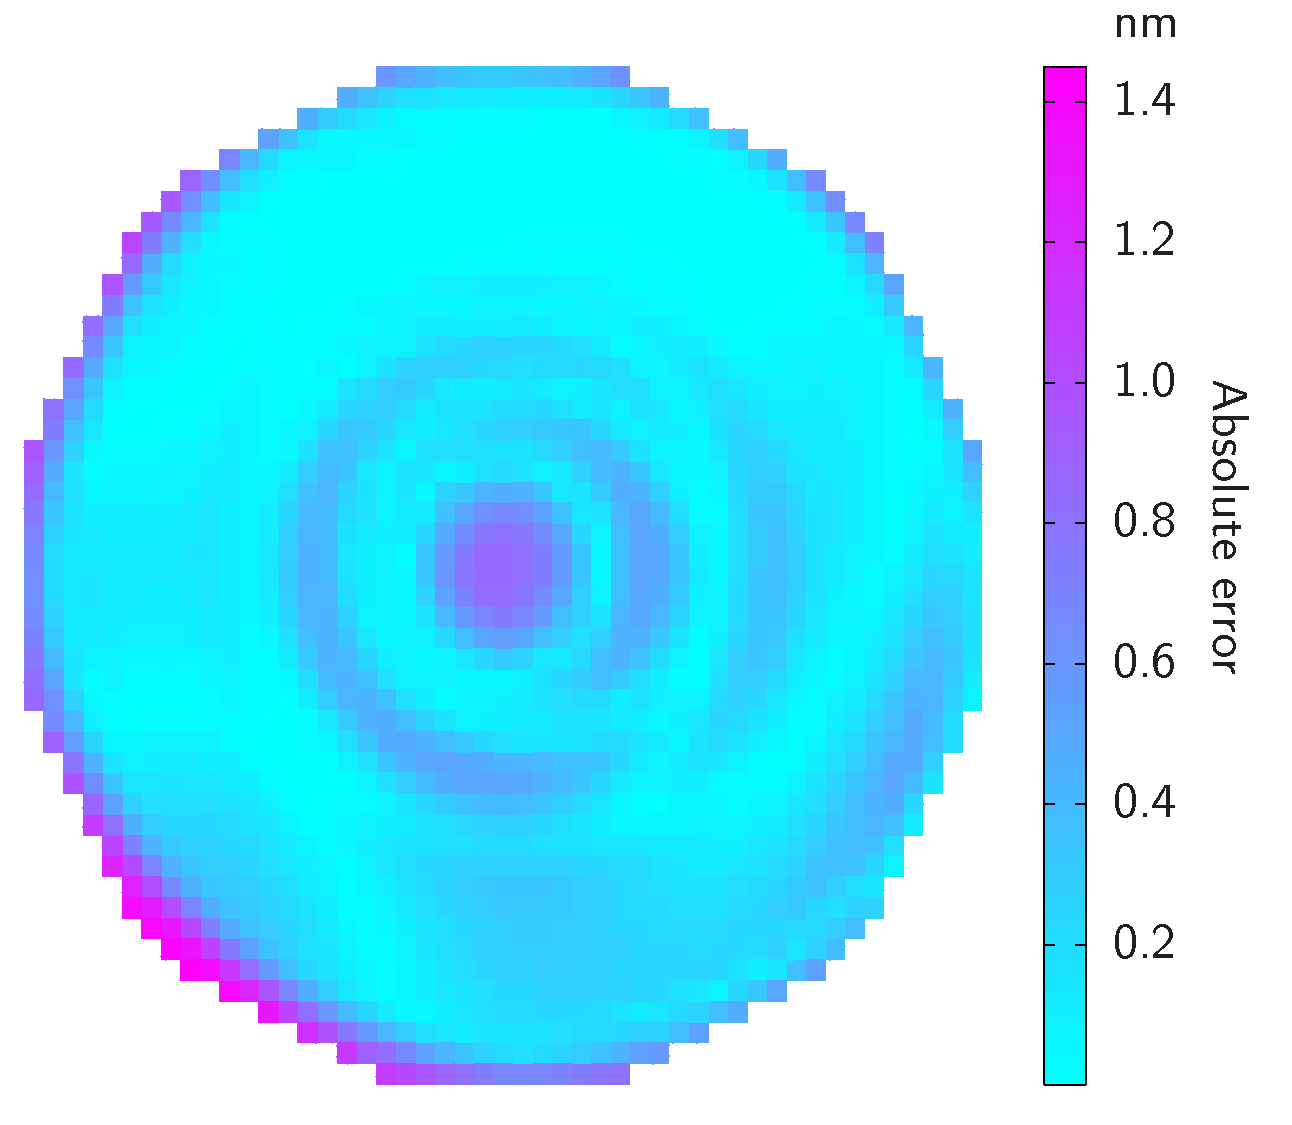
\includegraphics[width=0.6\linewidth]{include/figures/wafer-qoi-error.pdf}
  \caption{Distribution of the absolute error.}
  \flabel{wafer-qoi-error}
\end{figure}

In order to ensure that the experimental setup is adequate, let us first perform a detailed analysis of the results obtained for one particular example with the default configuration described earlier.
The true and inferred distributions of the \qoi\ are shown in \fref{wafer-qoi} where the normalized root-mean-square error (NRMSE) is below $2.8\%$, and the distribution of the absolute error across the wafer is visualized in \fref{wafer-qoi-error}. It can be seen that the framework produces a close match to the true value of the \qoi.
Now, we inspect the quality of the proposal distribution (recall \sref{bayesian-inference} and \sref{optimization}). To this end, we first plot (not shown) the posterior given in \eref{log-posterior} for each drawn sample and obtain a curve with $10^4$ points, which rapidly fluctuates around a constant level indicating that the constructed Markov chain vividly explores the underlying probability space.
Next, we calculate the acceptance rate of the Metropolis algorithm and find it to be $20$--$30\%$ on average, which agrees with the recommendations from the literature \cite{gelman2004}.
Another test, commonly used in statistics, to assess the quality of the proposal distribution is to depict side-by-side the posterior in \eref{log-posterior} and the tailored proposal in \eref{proposal} for each parameter, conditional on the other parameters being at their posterior modes. The curves (not shown) are nearly indistinguishable implying a high quality of the proposal. To sum up, the above observations suggest that the optimization and sampling procedures are fine-tuned.

\subsection{Number of Processing Elements on a Die}
In this subsection, we consider five platforms with the number of processing elements in each die $\nprocs$ equal to 2, 4, 8, 16, and 32 cores, respectively. The results are summarized in \tref{processing-elements}.
In this and the following tables, we report the optimization and sampling times (given in minutes) separately; also, the sampling time is given for two cases: sequential and parallel computing, which is followed by the total time and error.
The sequential sampling time is the most representative indicator of the computational complexity scaling as the number of samples is always fixed, and there is no parallelization; thus, we shall watch this value in most of the discussions below (highlighted in bold in the tables). The speedup due to parallel computing will be discussed later on.
\begin{table}[h]
  \centering
  \caption{Results for the number of processors $\nprocs$.}
  \begin{tabular*}{1\linewidth}{=l@{\hskip 4em}-r-r-r-r-r}
    \toprule
    Processing elements    & 2 & 4 & 8 & 16 & 32 \\
    \midrule
    \midrule
    Optimization time, m   & 2.67 & 3.34 &  5.20 &  7.37 & 13.85 \\
    \midrule
    \rowstyle{\bfseries}
    Sequential sampling, m & 3.71 & 4.60 &  6.03 &  8.92 & 14.77 \\
    Total time, m          & 6.38 & 7.94 & 11.23 & 16.29 & 28.62 \\
    \midrule
    Parallel sampling, m   & 0.98 & 1.18 &  1.58 &  2.51 & 5.30 \\
    Total time, m          & 3.65 & 4.52 &  6.78 &  9.88 & 19.15 \\
    \midrule
    NRMSE, \%              & 4.71 & 3.42 &  3.68 &  2.73 &  1.94 \\
    \bottomrule
  \end{tabular*}
  \tlabel{processing-elements}
  \vspace{-1em}
\end{table}


It can be seen in \tref{processing-elements} that all computational times grow with the number of processing elements. This behavior is expected as each processing element introduces additional complexity in the thermal system given by \eref{thermal-system}; more precisely, it leads to a larger number of thermal nodes $\nnodes$. Nevertheless, even for large examples, the timing is readily acceptable, taking into account the complexity of the inference procedure behind and the yielded accuracy.
An interesting observation can be made from the NRMSE: the error tends to decrease as the number of processing elements grows. The explanation is that, with each core, $\Data$ delivers more information to the inference to work with since the temperature profiles in $\Data$ are being collected for all the cores simultaneously.

\subsection{Number of Measured Dies}
In this subsection, we change the number of dies $\nrdies$ for which the measurement data are available in the input data set $\Data$ (correspondingly, $\ndies - \nrdies$ dies on the wafer are left unobserved). The considered scenarios are 1, 10, 20, 40, 80, and 160 measured dies. The results are reported in \tref{spatial-measurements}.
\begin{table}[h]
  \centering
  \caption{Results for the number of measured dies.}
  \begin{tabular*}{1\linewidth}{=l@{\hskip 4pt}-r-r-r-r-r-r}
    \toprule
    Measured dies   & 1 & 10 & 20 & 40 & 80 & 160 \\
    \midrule
    \midrule
    Optimization time, m   &  0.41 & 2.49 & 3.34 &  4.59 &  7.33 & 10.29 \\
    \midrule
    \rowstyle{\bfseries}
    Sequential sampling, m &  2.40 & 3.99 & 4.60 &  5.79 &  8.49 & 12.96 \\
    Total time, m          &  2.81 & 6.47 & 7.94 & 10.38 & 15.81 & 23.25 \\
    \midrule
    Parallel sampling, m   &  0.61 & 1.02 & 1.18 &  1.51 &  2.16 &  3.62 \\
    Total time, m          &  1.02 & 3.50 & 4.52 &  6.10 &  9.49 & 13.91 \\
    \midrule
    NRMSE, \%              & 30.49 & 4.40 & 3.42 &  1.09 &  0.85 &  0.67 \\
    \bottomrule
  \end{tabular*}
  \tlabel{spatial-measurements}
  \vspace{-1.5em}
\end{table}


We see that the more data the proposed framework needs to process, the longer the execution time, which is reasonable. The trend, however, is not as steep as the one in \tref{processing-elements} since the thermal system stays unchanged.
The error firmly decreases and drops below $4\%$ with around 20 measurement points, which is only $6.3\%$ of the total number of dies on the wafer.

This example is a great opportunity to emphasize that the posterior distribution provides a complete description of the uncertainty of the \qoi\ (recall also \sref{motivation}).
In \tref{spatial-measurements}, we have two extreme cases: one and 160 measurement points. It is reasonable to anticipate that the predictions are less accurate in the former case than those in the latter, and this is exactly what the NRMSE has revealed in \tref{spatial-measurements}.
Unfortunately, in reality, we do not have such a table to judge the accuracy of our predictions as the true values are unknown.
It is straightforward, however, to use the posterior draws to quantify the reduction of the prediction uncertainty with respect to the amount of available data.
The quantity to monitor here is the standard deviation of the constructed Markov chain: a lower level of this deviation implies a higher level of accuracy (certainty). In the experiment at hand, the reduction of the standard deviation with the traversal from one to 160 measured dies was found to be significant.

\subsection{Number of Temporal Measurements}
In this subsection, we sweep the number of moments of time $\nrsteps$ for which the measurement data are available in the input data set $\Data$ (correspondingly, $\nsteps - \nrsteps$ steps are discarded after $\model$ is evaluated for the input power profile $\profilePdyn$). The scenarios are 1, 10, 20, 40, 80, and 160 time moments. The results are aggregated in \tref{temporal-measurements}.
\begin{table}[h]
  \vspace{-1.5em}
  \centering
  \caption{Results for the number of temporal measurements.}
  \begin{tabular*}{1\linewidth}{=l-r-r-r-r-r-r}
    \toprule
    Temporal measurements  & 1 & 10 & 20 & 40 & 80 & 160 \\
    \midrule
    \midrule
    Optimization time, m   & 1.12 & 3.02 & 3.34 & 3.62 & 3.64 & 4.20 \\
    \midrule
    \rowstyle{\bfseries}
    Sequential sampling, m & 2.40 & 4.38 & 4.60 & 4.67 & 4.80 & 4.97 \\
    Total time, m          & 3.52 & 7.40 & 7.94 & 8.29 & 8.44 & 9.16 \\
    \midrule
    Parallel sampling, m   & 0.62 & 1.13 & 1.18 & 1.22 & 1.25 & 1.30 \\
    Total time, m          & 1.74 & 4.16 & 4.52 & 4.84 & 4.89 & 5.50 \\
    \midrule
    NRMSE, \%              & 7.48 & 2.72 & 3.42 & 1.83 & 2.34 & 1.32 \\
    \bottomrule
  \end{tabular*}
  \tlabel{temporal-measurements}
  \vspace{-0.5em}
\end{table}


As we see, the growth of the computational time is relatively low. One might have expected this time to be the same as the one for the spatial measurements since, formally, their influence on the dimensionality of $\Data$ is identical (recall $\mvT_\meas \in \real^{\nrdies \nrprocs \nrsteps}$). However, the meaning of the two numbers, $\nrdies$ and $\nrsteps$, is completely different, and, therefore, the way they manifest themselves in the algorithm is also different. Thus, the corresponding amounts of extra data are being treated differently leading to the discordant timing shown in \tref{spatial-measurements} and \tref{temporal-measurements}.
The NRMSE in \tref{temporal-measurements} is decreasing on average; however, the observed trend is less steady than the ones discovered before. The finding can be explained as follows. The distribution of the time moments in $\Data$ changes since these moments are kept evenly spaced across the corresponding time spans of the input power profiles. Some time moments can be more informative than the other. Consequently, more representative or less representative samples can end up in $\Data$ helping or misleading the inference procedure.
Based on \tref{spatial-measurements} and \tref{temporal-measurements}, we can also conclude that a larger number of spatial measurements is more advantageous for the inference than a larger number of temporal measurements.

\subsection{Deviation of the Measurement Noise}
In this subsection, we vary the standard deviation of the noise in the input data set $\Data$ within the set $\{ 0, 0.5, 1, 2 \}$ (in Kelvins). Note that the corresponding prior distribution in \eref{sigma2-noise-prior} is kept unchanged. The results are given in \tref{noise-deviation}.
\begin{table}[h]
  \centering
  \caption{Results for the level of the measurement noise.}
  \begin{tabular*}{1\linewidth}{=l@{\hskip 5.5em}-r@{\hskip 2em}-r@{\hskip 2em}-r@{\hskip 2em}-r}
    \toprule
    Deviation of the noise & 0, K & 0.5, K & 1, K & 2, K \\
    \midrule
    \midrule
    Optimization time, m     & 5.08 & 3.73 & 3.34 & 3.19 \\
    \midrule
    \rowstyle{\bfseries}
    Sequential sampling, m   & 4.76 & 4.70 & 4.60 & 4.71 \\
    Total time, m            & 9.84 & 8.43 & 7.94 & 7.90 \\
    \midrule
    Parallel sampling, m     & 1.19 & 1.17 & 1.18 & 1.18 \\
    Total time, m            & 6.27 & 4.91 & 4.52 & 4.37 \\
    \midrule
    NRMSE, \%                & 0.02 & 2.71 & 3.42 & 4.05 \\
    \bottomrule
  \end{tabular*}
  \tlabel{noise-deviation}
  \vspace{-1em}
\end{table}


Reasonable enough, the sampling time is approximately constant; however, we observe an increase of the optimization time with the decrease of the noise level, which can be ascribed to wider possibilities of perfection for the optimization procedure.
A more important observation, revealed by this experiment, is that, in spite of the fact that the inference operates on indirect and drastically incomplete data, a thoroughly calibrated equipment can considerably improve the quality of predictions.
However, even with a high level of noise of two degrees---meaning that all measurements fall on the band of $8~\text{K}$ wide around the true values with probability more than $0.95$---the NRMSE is still only $4\%$.

\subsection{Sequential vs. Parallel Sampling}
In this subsection, we summarize the results of the sequential and parallel  sampling strategies (see \sref{sampling}).
In the non-parallel Metropolis algorithm, the optimization time is typically smaller than the time needed to draw posterior samples.
The situation changes when parallel computing (with four processors, in our case) is utilized. The sampling time decreases by 3.81 times on average, which indicates good parallelization properties of the chosen sampling strategy.
The overall speedup, \ie, including the optimization part, ranges from 1.49 to 2.75 with the average value of 1.77 times, which can be pushed even further using more parallel processes.
